\chapter{Figuras}
\label{cha:figuras}



Lo primero que tienes que aprender sobre las figuras en \LaTeX{} es una máxima de desarrollo personal: aprende a soltar, a no querer el control. Y no, no es broma. \LaTeX{} decidirá por ti el lugar óptimo para colocar una figura dentro de la página.

Ahora repite lo difícil conmigo: ``Eso no está mal''.

Lo segundo que tienes que aprender es que la palabra ``figura'' incluye imágenes (jpg, png, eps, y otras), tablas, dibujitos creados con \LaTeX{}, y muchas cosas más. Pero, despacio, empecemos por una directiva primaria que jamás debes ignorar.



\section{Evita referencias de lugar}
\label{sec:evita_referencias_de_lugar}



Una de mis más grandes frustraciones con \LaTeX{} al inicio fue que hacía lo que quería con las imágenes, las colocaba en todo lugar menos donde yo tenía la intención de que estuvieran. Eso era porque sentía que no podía escribir algo como lo siguiente:

\begin{displayquote}
Podemos observar los resultados en la siguiente figura:

[Y luego... nada]
\end{displayquote}

\LaTeX{} decidía que la imagen se veía mejor en la parte superior de la página, o como tres páginas más abajo. Después de mucho trabajo personal, y estudios en \LaTeX{}, he llagado ha perdonarlo. Gracias a ello, en este capítulo puedo enseñarte que \LaTeX{} tiene su forma particular de determinar qué va dónde, a pesar de las instrucciones o sugerencias que tú le puedas dar en código.

Si vienes de Microsoft Word, como yo venía en ese entonces, deseas una solución con algún comando que permita hacer la imagen flotante para poder ignorar los márgenes del documento y colocar la imagen donde quieres específicamente.

Y, aunque sí hay paquetes para hacerlo, esa no es la manera adecuada para trabajar en \LaTeX{}, porque te estarías concentrando en el formato y no en el contenido. Además, tras una revisión de tu asesor (de las tantas), donde te hace eliminar tres hojas de relleno y meter más datos, ¿crees que habrá valido de algo tu esfuerzo por pelear la posición de una imagen que ha cambiado de lugar?

Lo que sugiero es reescribir la referencia a una imagen de la siguiente manera:

\begin{displayquote}
% Para escribir corchetes después de una instrucción en LaTeX,
% agrupar dentro de llaves: https://tex.stackexchange.com/a/305170
{[La imagen con |\label{imagen_ficticia}| puede estar áquí]}

Los resultados se muestran en la figura |\ref{imagen_ficticia}|.

[La imagen con |\label{imagen_ficticia}| puede estar áquí]
\end{displayquote}

Así ya no importa si la imagen está arriba, abajo, o en otra página, el lector la buscará. Obviamente, la referencia no puede estar tan lejos, y llegará el momento de colocar mejor las imágenes y tablas, pero mientras el trabajo está en proceso no hay necesidad de reacomodar nada.

Cambia tu manera de referenciar las figuras y todo será más fácil.



\section{Figuras}
\label{sec:figuras}


\LaTeX{} tiene un entorno llamado \texttt{figure}, que sirve básicamente para agregar una leyenda y un numerito a lo que dicho entorno contenga. Incluso puedo crear una figura sin agregar una imagen, como se muestra en la figura \ref{fig:figura_vacia} (¿ves? acabo de referenciar por etiqueta, no por ubicación).

\begin{figure}[ht!]
	\caption{¿Una figura vacía?}
	\label{fig:figura_vacia}
\end{figure}

Para ello utilicé el código del listado \ref{lst:figura_vacia}. Cuatro líneas de código son suficientes para que nos duela la cabeza dos veces (al menos, si nadie te explicara lo que sucede).

\begin{lstlisting}[style=latex,caption={Código para una figura vacía.},label=lst:figura_vacia]
\begin{figure}[ht!]
	\caption{¿Una figura vacía?}
	\label{fig:figura_vacia}
\end{figure}
\end{lstlisting}



\subsection{Indicador de ubicación}
\label{sub:indicador_de_ubicacion}



El primer dolor de cabeza ocurre gracias al valor que está entre corchetes en la primera línea del listado \ref{lst:figura_vacia}. En la sección \ref{sec:entornos} aprendimos que el contenido entre corchetes es un argumento cuyo propósito es modificar el contenido del entorno de alguna manera. En este caso, esos tres caracteres, \texttt{ht!}, que parecen inocuos:

\begin{lstlisting}[style=latex,numbers=none]
\begin{figure}[ht!]
\end{lstlisting}

\noindent corresponden al argumento \emph{indicador de ubicación}... que más o menos se refiere a dónde irá colocada la figura.

¿Por qué \emph{más o menos}? Porque este argumento es una \emph{sugerencia} de dónde deben ir colocados los \emph{flotantes}...



\subsection{Elementos flotantes}
\label{sub:elementos_flotantes}



Discúlpame, esto se salió de control muy rápido. Aunque nos podemos poner muy técnicos con esto de la ubicación de las figuras, trataré de tocar solo lo necesario. Los entornos \texttt{figure} y \texttt{table} se conocen como \emph{floats} (``elementos flotantes'', o solo ``flotantes'' en este texto) y lo que eso significa, de una manera simplificada, es esto:

\begin{displayquote}
Un flotante es un elemento que rompe el flujo normal del texto en \LaTeX{} y que, debido a esto, se le debe asignar una ubicación siguiendo ciertas reglas.
\end{displayquote}

De cierta manera, esto de la ubicación de flotantes es como el DIF\footnote{\emph{Desarrollo Integral de las Familias} es una organización mexicana que se encarga, entre otras cosas, de gestionar la adopción de niños.}: un flotante es un niño en busca de un hogar, y tu indicador de ubicación es la familia que lo va a adoptar. Ahora bien, hay muchas familias, y muchos niños, y el DIF revisa las aplicaciones para saber qué niño se va con cuál familia. En última instancia, no es la elección ni del niño ni de la familia si la adopción se realiza a gusto de todos.

Es decir, tú puedes sugerirle a \LaTeX{} dónde quieres que vaya tu figura (imagen, tabla...) pero siempre \LaTeX{} va a tener la decisión final. Si quieres una discusión más profunda, puedes leer el artículo en \cite{bib:figures_float}.

Como ejemplo de regla, digamos que tienes una página con texto que cubre el 51\%. Luego quieres insertar una imagen que ocupa el 50\% de la página. Para \LaTeX{}, $51 + 50$ es más del 100\% del espacio disponible en la hoja y su conclusión es inequívoca: más del 100\% significa que no cabe la imagen en la página actual, y te la mandará a la siguiente.

Puedes pelear todo lo que quieras, pero \LaTeX{} sigue sus reglas. Y, vamos, ¿cómo puedes ganarle a las matemáticas? Volvamos al indicador.



\subsection{Valores del indicador de ubicación}
\label{sub:valores_del_indicador_de_ubicacion}



Los valores posibles de este indicador se definen en la tabla \ref{tab:indicador_ubicacion} (siendo este otro ejemplo más de referencia por etiqueta, no por ubicación espacial).

\begin{table}[ht]
	\centering
	\begin{tabular}{cl}
		\hline
		\textbf{Parámetro} & \multicolumn{1}{c}{\textbf{Posición}}                         \\
		\hline
		\texttt{h}         & Aquí... por favor, y si es posible.                           \\
		\texttt{t}         & En la parte superior de la página (del inglés \emph{top}).    \\
		\texttt{b}         & En la parte inferior de la página (del inglés \emph{bottom}). \\
		\texttt{p}         & Colocar en una página especial para flotantes.                \\
		\texttt{!}         & Ignorar los parámetros que \LaTeX{} considera buenos.         \\
		\texttt{H}         & Sin comentarios...                                            \\
		\hline
	\end{tabular}
	\caption{Posibles valores del indicador de ubicación.} % Leyenda de la tabla.
	\label{tab:indicador_ubicacion}
\end{table}

No obstante, hay que considerar que el orden de evaluación del argumento (lo que escribes entre corchetes) no es tal y como lo escribes. Es decir, no evalúa la \texttt{h}, luego la \texttt{t}, y al final el \texttt{!}, sino que sigue la siguiente lista de prioridad:
\begin{itemize}
	\item Si hay un \texttt{!} presente, \LaTeX{} medio ignorará algo de su buen juicio en tu beneficio para tratar de poner la imagen justo en el lugar donde se encuentra en el código (no necesitas los detalles, pero si los quieres puedes consultar \cite{bib:figures_float}).
	\item Si no hay un \texttt{!}, enseguida buscará un \texttt{h}, para \emph{tratar} de colocar la figura justo donde tú la quieres (aunque con menos vehemencia que con un \texttt{!}).
	\item De ahí, busca la \texttt{t}, para tratar de ubicar la figura en la parte superior de la página.
	\item Al final revisa buscando la \texttt{b}, para colocar la figura en la parte inferior.
\end{itemize}

¿Y qué hay del valor \texttt{p}? Hace referencia a una página dedicada a flotantes, misma que generalmente crea \LaTeX{} cuando no sabe qué más hacer con tus figuras rebeldes.

¿Y el valor \texttt{H}? Es un valor que requiere del paquete \texttt{float} para funcionar, y que no recomiendo porque puede ignorar algunas cuantas reglas más de \LaTeX{} para acomodar tu figura donde tú la pides, pero eso puede terminar resultando desagradable visualmente. Si aún así gustas utilizarlo, puedes leer \cite{bib:float} para aprender sobre el paquete \texttt{float} y el significado del valor \texttt{H}. De nuevo, no considero que lo valga.

En mi opinión, el uso de \texttt{ht!} (o \texttt{!ht} o \texttt{t!h}, da igual) es suficiente para la mayoría de los casos. Y, si no es así, es mejor modificar un poco el contenido para que el documento se vea bien, en lugar de pelear con los flotantes.

Suficiente de la ubicación: ya sabemos qué significa \texttt{ht!} y por qué se utiliza. Vayamos al segundo dolor de cabeza, te prometo que es mucho menor que este que acabamos de pasar.



\subsection{Etiquetas en figuras}
\label{sub:etiquetas_en_figuras}



En la sección \ref{sec:etiquetas_y_referencias} aprendimos que una |\label| te puede dar la referencia a una sección. La misma instrucción puede ser aplicada a una figura, con una salvedad: debe estar incluída \textbf{después} de la |\caption| (leyenda) de la figura, o algo raro pasará con la referencia.

Como un primer ejemplo, tenemos de referencia la figura \ref{fig:figura_vacia} (y esta mención es la prueba de que su numerito asociado funciona). Si ahora creamos una segunda figura vacía, pero colocando la |\label| antes que la |\caption| como muestra el listado \ref{lst:figura_vacia_2}, la referencia hecha con |\ref{fig:figura_vacia_2}| no presenta un número: ``figura \ref{fig:figura_vacia_2}''. ¿Qué pasó aquí?

\begin{figure}[ht!]
	\label{fig:figura_vacia_2}
	\caption{Una segunda figura vacía.}
\end{figure}

\begin{lstlisting}[style=latex,caption=Código para la segunda figura vacía.,label=lst:figura_vacia_2]
\begin{figure}[ht!]
	\label{fig:figura_vacia_2}
	\caption{Una segunda figura vacía.}
\end{figure}
\end{lstlisting}

En mi inocencia, creí que mientras estuviera dentro del entorno \texttt{figure}, la referencia se haría correctamente, pero \LaTeX{} dice que no. Adicional a no imprimir el valor correcto, recibimos dos advertencias cortesía del compilador. La primera,

\begin{lstlisting}[style=advertencias]
Package caption Warning: \label without proper reference on input line 167.
\end{lstlisting}

\noindent sobre el |\caption| en el entorno \texttt{figure}, por tratar de hacer un |\label| antes de que exista un |\caption|; y la segunda,

\begin{lstlisting}[style=advertencias]
LaTeX Warning: Reference `fig:figura_vacia_2' on page 25 undefined on input line 171.
\end{lstlisting}

\noindent al tratar de usar la etiqueta con |\ref|, cuando hubo errores para crearla.

Sigamos con otro ejemplo, haciendo otra figura vacía (listado \ref{lst:figura_vacia_3}). En esta nueva figura se incluyen dos etiquetas, que al usar la instrucción |\ref| dan los números \ref{fig:figura_vacia_3} para |\ref{fig:figura_vacia_3}| mientras que la segunda etiqueta muestra el valor de \ref{fig:figura_vacia_3_adicional} (para |\ref{fig:figura_vacia_3_adicional}|).

\begin{figure}[ht!]
	\caption{Tercera figura vacía.}
	\label{fig:figura_vacia_3}
	\label{fig:figura_vacia_3_adicional}
\end{figure}

Con este ejemplo podemos concluir tres cosas:
\begin{enumerate}
	\item La instrucción |\caption| genera bien el número de referencia para la segunda figura, porque la tercera figura tiene su numeración correcta.
	\item Eso nos dice que la referencia es lo que no funciona, porque no imprime el número de la segunda figura vacía (se tiene acceso al número solo después asignar un |\caption| a la figura).
	\item Por último, que dos etiquetas diferentes sobre el mismo elemento apuntan al mismo elemento.
\end{enumerate}

\begin{lstlisting}[style=latex,caption=Código para la tercera figura vacía.,label=lst:figura_vacia_3]
\begin{figure}[ht!]
	\caption{Tercera figura vacía.}
	\label{fig:figura_vacia_3}
	\label{fig:figura_vacia_3_adicional}
\end{figure}
\end{lstlisting}

De hecho, gracias a ese último punto podemos concluir que es el comando |\caption|, y no el entorno \texttt{figure}, el que define la referencia. ¿Eso quiere decir que si metemos dos |\caption| en un \texttt{figure} tendrémos dos figuras? Veamos.\newline

\begin{figure}[ht!]
	\caption{Cuarta figura vacía.}
	\label{fig:figura_vacia_4}
	\caption{Cuarta figura vacía, pero segunda leyenda.}
	\label{fig:figura_vacia_4_2}
\end{figure}

En terminos de código, como se muestra en el listado \ref{lst:figura_vacia_4}, sí. El entorno resultante cuenta con ``dos figuras'': |\ref{fig:figura_vacia_4}| muestra el número \ref{fig:figura_vacia_4} mientras que |\ref{fig:figura_vacia_4_2}| muestra el valor \ref{fig:figura_vacia_4_2}.

\begin{lstlisting}[style=latex,caption=Código para la cuarta figura vacía.,label=lst:figura_vacia_4]
\begin{figure}[ht!]
	\caption{Cuarta figura vacía.}
	\label{fig:figura_vacia_4}
	\caption{Cuarta figura vacía, pero segunda leyenda.}
	\label{fig:figura_vacia_4_2}
\end{figure}
\end{lstlisting}

De momento, el ejemplo carece de sentido, ¿por qué no colocar cada figura dentro de su propio entorno? ¿Por qué ésto no genera un error o una advertencia? Esto solo fue un ejemplo entender el funcionamiento de \LaTeX{}, para explicar por qué si colocas un |\label| antes del |\caption| no se imprime la referencia. Ya discutiremos la lógica un poco más adelante.

Con esto fuera del camino, creemos imágenes con \LaTeX{}. Sí, crear.



\section{El entorno \texttt{picture}}
\label{sec:el_entorno_picture}



El entorno \texttt{picture} es un entorno que sirve para generar diagramas o imágenes simples en tu documento \cite{bib:overleaf_picture}. Ventajas... solo una: el resultado va a tener una calidad inigualable porque es realizado con vectores y se ve bien con cualquier nivel de zoom. ¿Desventajas? La poca practicidad de tener que dibujar mediante instrucciones y coordenadas (ah, los recuerdos de AutoCAD).

Como ejemplo de dibujo realizado con instrucciones en un entorno \texttt{picture} tenemos el rectángulo de la figura \ref{fig:picture_rectangulo}, cuyo código se muestra en el listado \ref{lst:picture_rectangulo}.

\begin{figure}[ht!]
	\setlength{\unitlength}{1mm} % Selección de unidad de medida.
	\centering % La figura se centra
	\begin{picture}(100, 20)  % ancho * alto
		\put(0, 0){\line(0,1){20}}
		\put(100, 20){\line(-1,0){100}}
		\put(0,0){\line(5,1){100}}
		\put(100, 20){\line(0,-1){20}}
		\put(0, 0){\line(1,0){100}}
	\end{picture}
	\caption{Rectángulo vacío con \texttt{picture}.} % Leyenda de la figura.
	\label{fig:picture_rectangulo}
\end{figure}

\begin{lstlisting}[style=latex,numbers=left,label=lst:picture_rectangulo,caption={Código para crear un rectángulo con \LaTeX{}.}]
\begin{figure}[ht!]
	\setlength{\unitlength}{1mm} % Selección de unidad de medida.
	\centering % La figura se centra
	\begin{picture}(100, 20)  % ancho * alto
		\put(0, 0){\line(0,1){20}}
		\put(100, 20){\line(-1,0){100}}
		\put(0,0){\line(5,1){100}}
		\put(100, 20){\line(0,-1){20}}
		\put(0, 0){\line(1,0){100}}
	\end{picture}
	\caption{Rectángulo vacío con \texttt{picture}.} % Leyenda de la figura.
	\label{fig:picture_rectangulo}
\end{figure}
\end{lstlisting}

La primera línea del listado \ref{lst:picture_rectangulo} abre un entorno \texttt{figure}, que cierra en la línea 13, para contener todas las instrucciones con las que realizamos el rectángulo, además de su |\caption| (línea 11) y |\label| (línea 12).

Antes de empezar a dibujar con \LaTeX{} es necesario establecer la unidad de medida, que es a lo que equivaldrá cada unidad del entorno \texttt{picture} ya en papel. Para evitar confusiones, lo más conveniente es hacer la unidad de medida de un milímetro (o de alguna otra unidad del sistema internacional), con el comando

\begin{lstlisting}[style=latex]
\setlength{\unitlength}{1mm}
\end{lstlisting}

\noindent definido en la línea 2. En la línea 3 se usa la instrucción |\centering| para centrar el contenido. Posteriormente se abre el entorno \texttt{picture}, en la línea 4, recibiendo sus dimensiones en ancho por alto (de la unidad de medida previamente establecida). Si queremos un rectángulo de 10 centímetros de largo por 2 centímetros de alto, usamos la instrucción

\begin{lstlisting}[style=latex]
\begin{picture}(100, 20)
\end{lstlisting}

\noindent porque la unidad de medida es \texttt{1mm}. Para dibujar necesitamos establecer el punto desde donde va a partir el trazo (línea, círculo, rectángulo), siendo la esquina inferior izquierda el punto \texttt{(0, 0)}. En el caso de nuestro rectángulo, la esquina superior derecha está en el punto \texttt{(100, 20)}.

El primer lado del rectángulo lo podemos dibujar con una línea que parte del origen (con |\put{0, 0}|), tiene una longitud de \texttt{20mm}, y va en dirección \texttt{(0, 1)}, porque no avanza horizontalmente pero sí verticalmente. Es decir, el primer trazo del rectángulo se coloca con:

\begin{lstlisting}[style=latex]
\put(0, 0){\line(0,1){20}}
\end{lstlisting}

Hablemos un poco sobre por qué la instrucción |\line(5,1){100}| en la línea 7 muestra una diagonal de esquina a esquina en nuestro rectángulo. La dirección se da con un punto $(x, y)$ que \LaTeX{} usa para calcular la pendiente. No todos los grados son válidos, y solo hay 25 posibles valores si tomamos un solo cuadrante \cite{bib:picture_line}, porque los valores de $x$ y $y$ solo pueden ser enteros, coprimos\footnote{Números primos entre sí, o no divisibles entre sí, o números cuyo máximo común divisor es 1.}, y menores que 7. Complicado, lo sé. Volviendo, la diagonal se creó con:

\begin{lstlisting}[style=latex]
\put(0,0){\line(5,1){100}}
\end{lstlisting}

\noindent porque avanzamos cinco veces más en $x$ que en $y$, y los \texttt{100} que definen la longitud no corresponden a la longitud de la línea sino al desplazamiento horizontal (un total de \texttt{100} unidades en $x$, con un ángulo dado por la relación \texttt{5:1}).

Una vez que hemos evaluado la diagonal, las demás líneas son triviales. El código |\put(0, 0){\line(0,1){20}}| corresponde a una línea que se desplaza \texttt{20} unidades en $y$, hacia arriba, a partir del punto origen.

También podemos desplazarnos con números negativos, los cuales indican un cambio de dirección. Negativo en $x$ quiere decir a la izquierda, mientras que negativo en $y$ quiere decir hacia abajo. Si queremos dibujar la línea superior a partir de la esquina en \texttt{(100, 20)} podemos utilizar la dirección \texttt{(-1, 0)}:

\begin{lstlisting}[style=latex]
\put(100, 20){\line(-1,0){100}}
\end{lstlisting}

Por cierto, ¿mencioné que había una instrucción para crear rectángulos? En lugar de crear cuatro líneas pudimos crear el rectángulo con una sola instrucción: |\framebox(100, 20){}|. Pero, ¿dónde quedaría la diversión de la docencia?




\subsection{Esquema de \LaTeX{}}
\label{sub:esquema_de_latex}



¿Recuerdas la figura \ref{fig:esquema_latex}, el esquema de \LaTeX{} que vimos en la introducción?

\begin{figure}[ht!]
	\setlength{\unitlength}{3.5mm} % selección de unidad de medida.
\centering % La figura se centra
\begin{picture}(32, 5)  % ancho * alto
	% Las coordenadas del comando "put" son en base a la esquina inferior izquierda.
	\put(9,0.5){\framebox(14,4){Instrucciones en \LaTeX}}
	\put(1.5,2.5){\vector(1,0){7.5}}
	\put(23,2.5){\vector(1,0){7.5}}
	\put(1.5,3){Nuestro texto}
	\put(24,3) {PDF final}
\end{picture}
\end{figure}

Sí, el verdadero rostro de la figura \ref{fig:esquema_latex} es el código del listado \ref{lst:picture_esquema}. Antes de siquiera entrar al código podemos discernir seis elementos que necesitamos agregar: un recuadro, dos flechas, y tres cajas de texto.

Contrario al sabio caso del rectángulo, cuya unidad era de \texttt{1mm}, el esquema de \LaTeX{} adoptó como unidad de medida los \texttt{3.5mm} (línea 2 del listado \ref{lst:picture_esquema}). Eso complica un poco las operaciones porque ahora hay que calcular. La línea 4 nos dice que el espacio que tomará la figura es de \texttt{32$\times$5} unidades, lo que implica un tamaño de \texttt{112mm$\times$17.5mm} (porque la unidad base ahora mide \texttt{3.5mm}... matemáticas).

\begin{lstlisting}[style=latex,numbers=left,label=lst:picture_esquema,caption={Código de la figura \ref{fig:esquema_latex}.}]
\begin{figure}[ht!]
	\setlength{\unitlength}{3.5mm} % Selección de unidad de medida.
	\centering % La figura se centra
	\begin{picture}(32, 5)  % ancho * alto
		% Las coordenadas de \put son en base a la esquina inferior izquierda
		\put(9,0.5){\framebox(14,4){Instrucciones en \LaTeX}}
		\put(1.5,2.5){\vector(1,0){7.5}}
		\put(23,2.5){\vector(1,0){7.5}}
		\put(1.5,3){Nuestro texto}
		\put(24,3) {PDF final}
	\end{picture}
\end{figure}
\end{lstlisting}

El rectángulo será de un alto de \texttt{4} unidades, por lo que para estar centrado verticalmente nos sobra un margen de \texttt{0.5}. Si queremos centrar horizontalmente tenemos que considerar que si la longitud es de \texttt{14} unidades, entonces sobran \texttt{18} unidades, para ser distribuidas \texttt{9} a cada lado. Sí, esas dos operaciones para decir que el punto de inicio de nuestro rectángulo de tamaño \texttt{(14, 4)} es \texttt{(9, 0.5)} para estar centrado en un lienzo de \texttt{(32, 5)}. Que, por cierto, ninguno de esos números es su tamaño impreso de \texttt{49mm$\times$14mm} (y sí, puedes medirlo con una regla).

Las ``flechitas'' se hacen mediante la instrucción |\vector| y reciben los mismos parámetros que una |\line|. Para que estuvieran centradas se colocaron en el punto \texttt{2.5} en $y$. Su posición horizontal depende de la longitud y, como el rectángulo empieza en \texttt{9}, la flecha izquierda debe iniciar en \texttt{9 - longitud}, mientras que la flecha derecha empieza en \texttt{9+14} (coordenada inicial más largo del rectángulo). Su posición la definimos como:

\begin{lstlisting}[style=latex]
% Formato para realizar los cálculos de la flecha izquierda.
\vector(9 - longitud, 2.5){longitud}
% Con longitud de 7.5:
\vector(1.5, 2.5){7.5}
% Formato para flecha derecha:
\vector(9 + 14, 2.5){longitud}
% Con longitud de 7.5:
\vector(23, 2.5){7.5}
\end{lstlisting}

La posición del texto se deja como ejercicio al lector.



\subsection{Figuras \emph{.tex}}
\label{sub:figuras_emph}



Las figuras hechas con \texttt{picture} pueden crecer en instrucciones y convertirse en monstruos. Es aconsejable colocar las instrucciones de la figura en un archivo separado y guardarlo junto con el resto de las imágenes. Esto nos permitirá saber que el archivo \texttt{tex} corresponde a una imagen.

En el caso del esquema podemos realizar la separación de las instrucciones del listado \ref{lst:img_esquema_tex}. Recomiendo no incluir la |\caption| ni la |\label| por si se desea utilizar la ``imagen'' en múltiples instancias (redefinir una etiqueta marca una advertencia).

\begin{lstlisting}[style=latex,label=lst:img_esquema_tex,caption={Código del archivo \texttt{esquema\_latex.tex}.}]
\setlength{\unitlength}{3.5mm} % Selección de unidad de medida.
\centering % La figura se centra
\begin{picture}(32, 5)  % ancho * alto
	% Las coordenadas de \put son en base a la esquina inferior izquierda.
	\put(9,0.5){\framebox(14,4){Instrucciones en \LaTeX}}
	\put(1.5,2.5){\vector(1,0){7.5}}
	\put(23,2.5){\vector(1,0){7.5}}
	\put(1.5,3){Nuestro texto}
	\put(24,3) {PDF final}
\end{picture}
\end{lstlisting}

Con ese archivo podemos actualizar la llamada a la imagen como:

\begin{lstlisting}[style=latex]
\begin{figure}[ht!]
	\setlength{\unitlength}{3.5mm} % selección de unidad de medida.
\centering % La figura se centra
\begin{picture}(32, 5)  % ancho * alto
	% Las coordenadas del comando "put" son en base a la esquina inferior izquierda.
	\put(9,0.5){\framebox(14,4){Instrucciones en \LaTeX}}
	\put(1.5,2.5){\vector(1,0){7.5}}
	\put(23,2.5){\vector(1,0){7.5}}
	\put(1.5,3){Nuestro texto}
	\put(24,3) {PDF final}
\end{picture}
	\caption{Esquema de trabajo en \LaTeX.} % Leyenda de la figura.
	\label{fig:esquema_latex}
\end{figure}
\end{lstlisting}


~\newline
\indent Crear una imagen con código en \LaTeX{} es tedioso e innecesario, pero se justifica si quieres un documento de mayor calidad, tanto impresa como digital. Tu decisión. Si decides realizar dibujos con \LaTeX{}, procura buscar el paquete \texttt{TikZ} y ejemplos en la red \cite{bib:ejemplos_tikz}.



\section{Imágenes}
\label{sec:imagenes}



Puede que para estas alturas ya no te sorprenda tanto el hecho pero... \LaTeX{} no tiene así como que mucho soporte para imágenes de manera nativa. Tenemos que usar un paquete adicional, llamado \texttt{graphicx}. Ya sabes, preámbulo:

\begin{lstlisting}[style=latex,numbers=none]
\usepackage{graphicx} % Permite usar \includegraphics
\end{lstlisting}

Gracias a \texttt{graphicx} podemos insertar una imagen con el código mostrado en el listado \ref{lst:codigo_imagen}, donde solo la línea 3 es nueva: se usa |\includegraphics| para incluir una imagen, y su único argumento obligatorio corresponde al nombre del archivo. Dentro de los corchetes, como parámetro opcional, recibe el ancho de la imagen, que se establece al largo de la línea (con |\linewidth|).

\begin{lstlisting}[style=latex,numbers=left,caption={Código de la figura \ref{fig:overleaf_home}.},label=lst:codigo_imagen]
\begin{figure}[ht!]
	\centering
	\includegraphics[width=\linewidth]{img/overleaf_300ppi.png}
	\caption{Página principal de Overleaf.}
	\label{fig:overleaf_home}
\end{figure}
\end{lstlisting}

La línea 3 nos abre tres temas: la ventaja que supone referenciar por archivo, el directorio predeterminado, y las opciones de la imagen.



\subsection{Ventajas de agregar por archivo}
\label{sub:ventajas_de_agregar_por_archivo}



La sección \ref{sec:figuras} dejó un sabor un tanto amargo al saber que la ubicación de imágenes en una página era un proceso más allá de nuestro control, o algo bastante complicado si pretendemos modificarlo.

No obstante, llegaron las buenas noticias: ¡hay muchas ventajas en medio de este sufrimiento! Sí, claro, no es como Word que permite arrastrar y soltar, y todo se resuelve. No. Pero eso implica ventajas tremendas.

\subparagraph{El tamaño de archivo durante la edición es pequeño.\label{page:uso_subparrafos}} Sí. Un proyecto en \LaTeX{} es un conjunto de archivos. El archivo principal, un archivo por capítulo, y ahora resulta que también las imágenes se quedan aparte.

Eso implica que tú te puedes seguir ocupando de escribir en texto plano, en Overleaf o en Sublime Text, porque trabajar con una imagen, incluso de 20MB, solo implica unos pocos bytes del código que supone incluirla.

Si tienes cien imágenes de 1MB, tú en el editor sigues trabajando con 500 líneas de código (cinco por imagen), sin ver imapactado el desempeño.

¡No hay sufrimiento por periodos de carga del documento mientras escribes!

Esto no es por satanizar a Word o decir que es una mala herramienta\footnote{Para escribir una tesis de ingeniería sí considero que lo es, pero esa es otra historia.}, pero algunas veces al incluir una nueva imagen tienes que esperar a que se cargue en el documento, y hasta llegas a rezar porque esa inclusión no vaya a trabar Word y hacer que pierdas todo tu avance.

\subparagraph{¿Me equivoque de imagen? La cambio y recompilo.} Como \LaTeX{} incluye las imágenes por referencia, realmente no le importa si una imagen cambió o no entre compilación y compilación.

Eso implica que, si te equivocaste de imagen, basta con sobreescribir y recompilar. Los comandos |\caption| y |\label| siguen igual, y sus referencias no cambian. Por supuesto, si hubo mucha diferencia respecto a la imagen anterior, deberás cambiar el tamaño, pero representa muchos menos problemas que cambiar una imagen en Word.

\subparagraph{¿Imagen muy pesada? Bajo resolución y recompilo.} No solo puedes cambiar una imagen por otra. Si descubres que no hay diferencia entre la imagen si pesa 20MB o 2MB, puedes comprimir tu imagen y recompilar. Incluso si cambias un archivo bmp por un png, por temas de compresión, en código solo supone un cambio de extensión. No importa lo que le tengas que hacer a la imagen, a \LaTeX{} solo le importa que esté presente al momento de la compilación.

\subparagraph{Mejor control de versiones.} Aunque es un tema fuera del alcance de este libro, recomiendo que guardes tu tesis utilizando un sistema de versionado, como git. Hay varios servicios en línea que ofrecen repositorios privados gratuitos, como \href{https://bitbucket.org/}{BitBucket}. Puedes guardar los cambios en texto de tu tesis, independiente de las imágenes. En lugar de tener 20 copias de un documento de Word de 10MB cada una, con nombres como \emph{Copia\_20201130}, \emph{Respaldo\_20201131}, \emph{Respaldo\_2}, \emph{TesisFinal}, \emph{TesisFinalRevisada}, y más, esta segmentación permite guardar incrementalmente el texto plano de tu tesis, sin preocuparte por el peso de las imágenes o del PDF que se genera.



\subsection{Directorio de imágenes}
\label{sub:directorio_de_imagenes}



De manera predeterminada, \LaTeX{} lee las imágenes que se encuentran en el mismo directorio que el archivo que está siendo compilado. En un principio, eso puede sonar simple... pero ya separamos nuestra tesis en varios documentos, en la sección \ref{sec:separacion_en_archivos}. Entonces, ¿la imagen se busca desde el directorio del archivo principal o desde el directorio del archivo en el que se incluye la imagen? Si eso ya es demasiado confuso, recomiendo no liarse tanto y seguir la siguiente distribución:
\vspace{\topsep}
\dirtree{%
.1 /\DTcomment{Directorio raíz del proyecto}.
.2 ch\_intro.tex\DTcomment{Cada uno de los capítulos}.
.2 LaTeX para tesis de ingeniería.tex\DTcomment{Archivo principal del proyecto}.
.2 img\DTcomment{Directorio para almacenar las imágenes}.
.3 overleaf\_home.png\DTcomment{Cada una de las imágenes del proyecto}.
}
\vspace{\topsep}

Es decir, colocar todos los capítulos en el mismo directorio que el archivo principal para que no haya diferencia entre \texttt{img} e \texttt{./img} (como se menciona en \cite{bib:overleaf_inserting_images}). Como opción, dado que todas mis imágenes están en el subdirectorio \texttt{img}, podría configurar lo siguiente en el preámbulo:

\begin{lstlisting}[style=latex,numbers=none]
\graphicspath{ {img/} }
\end{lstlisting}

\noindent para incluir las imágenes con:

\begin{lstlisting}[style=latex,numbers=none]
\includegraphics[width=\linewidth]{overleaf.png}
\end{lstlisting}

\noindent lo que sería igual a \texttt{img/overleaf\_home.png} porque el valor de |\graphicspath| se añade al inicio de toda imagen incluida con la instrucción |\includegraphics|.

Puedes no configurar el subdirectorio de imágenes y siempre colocar el \texttt{img/} en cada inclusión de imagen, o configurar el parámetro para escribir un poco menos. Procede de la manera que consideres conveniente.



\section{Opciones de la imagen}
\label{sec:opciones_de_la_imagen}



Hay muchas cosas que podemos hacer con el paquete \texttt{graphicx} \cite{bib:package_graphicx}. Lo que aquí más nos importa es responder a la pregunta ``¿Cómo le digo a \LaTeX{} de qué tamaño quiero la imagen?'' Veamos las opciones.



\subsection{\texttt{scale}}
\label{sub:scale}



La opción \texttt{scale} determina el tamaño que la imagen tendrá en el documento en base al tamaño real de la imagen... al menos, esa es la teoría. Resulta que algunas imágenes no tienen en sus metadatos información sobre los puntos por pulgada (ppi, \emph{pixels per inch}), o no tienen los ppi adecuados. El estándar de impresión dice que una imagen debe contar con 300 ppi, y esa densidad es la que \LaTeX{} utiliza para sus cálculos con el parámetro |scale|. Es decir, \LaTeX{} asumirá que una imagen tiene 300ppi. Si no es así, los resultados pueden no ser los esperados.

Como ejemplo, la figura \ref{fig:overleaf_home_scale} muestra el mismo archivo que la figura \ref{fig:overleaf_home}, pero con el parámetro \texttt{scale=1} (código en el listado \ref{lst:figura_scale}). La densidad de ppi es menor a 300, lo que resulta en una imagen agrandada, con el efecto de la magnificación bastante visible.

\begin{lstlisting}[style=latex,caption=Uso de \texttt{scale=1}.,label=lst:figura_scale]
\begin{figure}[ht!]
	\centering
	\includegraphics[scale=1]{img/overleaf.png}
	\caption{Página principal de Overleaf, usando \texttt{scale=1}.}
	\label{fig:overleaf_home_scale}
\end{figure}
\end{lstlisting}

Otro escenario donde las cosas pueden ir mal es cuando la imagen excede el ancho de línea de la página y se sale de los márgenes del documento. Claro, la figura \ref{fig:overleaf_home_scale} se sale del documento, pero es por falta de resolución. Me refiero a que también puede pasar si incluyes una captura de pantalla de tu monitor 4K con escala igual a 1.

Volviendo a la imagen, hay formas de ajustar los ppi de una imagen, como se menciona en \cite{bib:stack_image_data}, pero algunas veces es mejor evitar tanto conflicto y optar por definir el tamaño de la imagen en términos del parámetro \texttt{width}.

\begin{figure}[ht!]
	\centering
	\includegraphics[scale=1]{img/overleaf.png}
	\caption{Página principal de Overleaf, usando \texttt{scale=1}.}
	\label{fig:overleaf_home_scale}
\end{figure}
\FloatBarrier



\subsection{\texttt{width}}
\label{sub:width}



Establecer el ancho nunca falla, aunque tal vez haya más unidades y valores de referencia de los que podemos digerir (véase \cite{bib:overleaf_units} y \cite{bib:latex_lengths}). Para efectos prácticos, diremos que solamente podemos poner las imágenes en milímetros (con \texttt{mm}) o centímetros (con \texttt{cm}), y eso si necesitas un valor absoluto.

Generalmente, es más práctico establecer el ancho de una imagen a través de longitudes de referencia, entre las que destacan:
\begin{itemize}
	\item |\linewidth|, para el ancho del texto en una línea,
	\item |\paperwidth|, para el ancho completo de la página (de lado a lado, pues),
	\item |\paperheight|, para el alto completo de la página.
\end{itemize}

Si establecemos la anchura de una imagen como |width=\linewidth|, estamos garantizando que no excederemos el ancho del texto (por lo tanto, nuestro documento se verá bonito).

También podemos utilizar esas longitudes como parte de operaciones aritméticas. Es decir, si escribimos |0.50\linewidth|, la imagen ocupará la mitad de la línea, como se muestra en la figura \ref{fig:overleaf_home_width_05}. Su código correspondiente es el listado \ref{lst:figura_width}.

\begin{lstlisting}[style=latex,caption=Uso de \texttt{width}.,label=lst:figura_width]
\begin{figure}[ht!]
	\centering
	\includegraphics[width=0.50\linewidth]{img/overleaf_300ppi.png}
	\caption{Página principal de Overleaf, al 50\% del ancho de línea.}
	\label{fig:overleaf_home_width_05}
\end{figure}
\end{lstlisting}

\begin{figure}[ht!]
	\centering
	\includegraphics[width=0.50\linewidth]{img/overleaf_300ppi.png}
	\caption{Página principal de Overleaf, al 50\% del ancho de línea.}
	\label{fig:overleaf_home_width_05}
\end{figure}



\subsection{\texttt{height}}
\label{sub:height}



Otra opción es establecer el tamaño de la imagen por medio del alto, para lo cual podemos utilizar las mismas unidades y longitudes de referencia que para el ancho. Y podemos combinar tanto |width| como |height| para la misma |\includegraphics|:

\begin{lstlisting}[style=latex]
\includegraphics[width=\linewidth,height=1.8cm]{img/overleaf_300ppi.png}
\end{lstlisting}

No obstante, definir tanto el ancho como el alto puede producir una imagen deformada, como se muestra en la figura \ref{fig:overleaf_home_height}.

\begin{figure}[ht!]
	\centering
	\includegraphics[width=\linewidth,height=1.8cm]{img/overleaf_300ppi.png}
	\caption{Página principal de Overleaf, con \texttt{width} y \texttt{height}.}
	\label{fig:overleaf_home_height}
\end{figure}



\subsection{\texttt{keepaspectratio}}
\label{sub:keepaspectratio}



Para evitar el resultado anterior existe la opción \texttt{keepaspectratio}, cuyo valor puede ser \texttt{false} o \texttt{true}. De manera predeterminada, es falso (y por eso pasó lo que pasó en la figura \ref{fig:overleaf_home_height}).

La figura \ref{fig:overleaf_home_height_aspect} supone un valor entre corchetes que incluye tres valores diferentes para la instrucción |\includegraphics|: \texttt{width}, \texttt{height}, y \texttt{keepaspectratio}. El listado \ref{lst:tres_valores_graphics} muestra cómo podemos dar un mejor formato visual a través de saltos de línea, aunque en efecto sigue siendo el mismo comando.

\begin{lstlisting}[style=latex,numbers=none,caption={Uso de \texttt{width}, \texttt{height}, y \texttt{keepaspectratio}.},label=lst:tres_valores_graphics]
\includegraphics[
	width=0.80\linewidth, height=1.8cm, keepaspectratio=true
]{img/overleaf_300ppi.png}
\end{lstlisting}

Ahora bien, si \LaTeX{} debe preservar el aspecto, y tiene tanto el ancho como el alto, ¿cuál de los dos números conserva? No hay una respuesta absoluta, sino que se basa en cálculos: la primer dimensión que llegue a su límite determinará la restante.

Es decir, en el caso de la figura \ref{fig:overleaf_home_height_aspect}, primero se llega a la altura máxima, haciendo que la anchura no llegue hasta el |\linewidth| esperado, manteniendo el aspecto.

\begin{figure}[ht!]
	\centering
	\includegraphics[width=\linewidth,height=1.8cm,keepaspectratio=true]{img/overleaf_300ppi.png}
	\caption{Página principal de Overleaf, con \texttt{width}, \texttt{height}, y \texttt{keepaspectratio}.}
	\label{fig:overleaf_home_height_aspect}
\end{figure}



\subsection{\texttt{angle}}
\label{sub:angle}



La última opción que veremos aquí es \texttt{angle}. Por supuesto, no son todas las opciones, pero para una guía exhaustiva tienes \cite{bib:package_graphicx}. La razón más común para usar \texttt{angle} es rotar una imagen que queremos mostrar en todo su esplendor... pero no cabe en el ancho de la hoja. Por fortuna, tenemos el alto, ¿no?

La figura \ref{fig:overleaf_home_angle} muestra la misma imagen que hemos usado todo este capítulo, rotada 90 grados en sentido antihorario producto de utilizar el argumento \texttt{angle=90}. También, para ser consistentes con el hecho de que la imagen ahora depende del alto del papel, la medida se cambió al 80\% del alto de la página.

Es importante recordar que |\paperheight| es toda la hoja, incluyendo márgenes, por lo que una imagen a todo lo alto se desbordaría (porque tenemos un margen en la parte superior de la página). El código de la figura \ref{fig:overleaf_home_angle} se muestra en el listado \ref{lst:graphics_angle}.

\begin{figure}[ht!]
	\centering
	\includegraphics[width=0.8\paperheight,angle=90]
		{img/overleaf_300ppi.png}
	\caption{Página principal de Overleaf, rotada 90 grados.}
	\label{fig:overleaf_home_angle}
\end{figure}

\begin{lstlisting}[style=latex,numbers=none,caption={Uso de \texttt{angle=90}},label=lst:graphics_angle]
\begin{figure}[ht!]
	\centering
	\includegraphics[width=0.8\paperheight,angle=90]{img/overleaf_300ppi.png}
	\caption{Página principal de Overleaf, rotada 90 grados.
	\label{fig:overleaf_home_angle}}
\end{figure}
\end{lstlisting}



\subsection{Entorno \texttt{sidewaysfigure}}
\label{sub:sidewaysfigure}



Hay un ligero problema con la figura \ref{fig:overleaf_home_angle}: su leyenda no rota junto con ella. Ese problema lo podemos resolver cargando el paquete \texttt{rotating} y usando su entorno \texttt{sidewaysfigure}, en lugar del \texttt{figure} regular.

El listado \ref{lst:sideways} muestra un ejemplo de código usando este entorno (imagen no incluida en el documento), en el que hay que destacar cuatro cosas:
\begin{enumerate}
	\item El entorno utilizado ahora es \texttt{sidewaysfigure} en lugar de \texttt{figure}.
	\item Se remueve la opción \texttt{angle} porque el entorno rota automáticamente la figura.
	\item Se remueve el indicador de posición porque el entorno tiene el valor \texttt{p}.
	\item Se usa el valor de \texttt{p} porque se asume que la imagen es muy grande para caber horizontalmente y por lo tanto abarcará toda la página.
\end{enumerate}

\begin{lstlisting}[style=latex,numbers=none,caption={Figura en entorno \texttt{sidewaysfigure}.},label=lst:sideways]
\begin{sidewaysfigure}
	\centering
	\includegraphics[width=0.8\paperheight]{img/overleaf_300ppi.png}
	\caption{Página principal de Overleaf, con \texttt{sidewaysfigure}.}
	\label{fig:overleaf_home_sideways}
\end{sidewaysfigure}
\end{lstlisting}



\FloatBarrier % Para contener la figura rotada.
\section{Advertencias de dimensiones}
\label{sec:advertencias_de_dimensiones}



Este documento tiene una advertencia gracias a la figura \ref{fig:overleaf_home_scale}, misma que se desborda de los márgenes, incluso del tamaño de la hoja. Al compilar, la bitácora mostrará una advertencia similar a la siguiente

\begin{lstlisting}[style=advertencias]
LaTeX Warning: Float too large for page by 1055.49106pt on input line 532.
\end{lstlisting}

\noindent por cada elemento que no se haya podido colocar correctamente. Lo que \LaTeX{} nos está diciendo es que no pudo acomodar la imagen dentro del espacio que tiene predefinido para el texto (la página menos los márgenes), y que muy posiblemente se ve fea.

No es un error, \LaTeX{} puede vivir con ello (por eso es una advertencia, y se marca con amarillo en este libro). Es solo una nota para que tú decidas si quieres hacer algo al respecto, o no.

\section{Subfiguras}
\label{sec:subfiguras}



Ahora que ya entendimos las figuras, es tiempo de pasar a las subfiguras. ¿Qué es eso? Varias imágenes, con su propia referencia, dentro de la misma figura. Como posiblemente ya sospechas, sí, necesitamos otro paquete en el preámbulo:

\begin{lstlisting}[style=latex,numbers=none]
\usepackage{subcaption} % Permite crear subfiguras.
\end{lstlisting}

El código de esto se vuelve un poco más complejo, porque ahora ya tenemos la figura \ref{fig:figure_subfigure}, la cual contiene las figuras \ref{fig:sub_1} y \ref{fig:sub_2}. No obstante, analicemos parte por parte del listado \ref{lst:figura_subfiguras}.

\begin{figure}[ht!]
	\begin{subfigure}[ht!]{.5\linewidth} % Ancho del contenedor de la imagen
		\centering
		% Primera imagen
		% Este ancho es de la imagen dentro del contenedor de la subfigura.
		\includegraphics[width=.95\linewidth]{img/overleaf_boton_log_300ppi.png}
		\caption{Lado izquierdo.}
		\label{fig:sub_1}
	\end{subfigure} % No debe haber líneas vacias entre esta y la siguiente subfigura
	~ % O la siguiente subfigura se mostrará debajo, en lugar de a un lado.
	\begin{subfigure}[ht!]{.5\linewidth}
		\centering
		% Segunda imagen
		\includegraphics[width=.95\linewidth]{img/overleaf_boton_cache_300ppi.png}
		\caption{Lado derecho.}
		\label{fig:sub_2}
	\end{subfigure}
	\caption{Figura con dos subfiguras.}
	\label{fig:figure_subfigure}
\end{figure}

Las líneas 1, y de la 18 a la 20, ya las conocemos. Es una figura como tal. Si revisamos las líneas de la 2 a la 9, una subfigura sigue el mismo formato que una figura: instrucción de centrado, inclusión de imagen, leyenda, y etiqueta. ¿Cuál es la diferencia, entonces?

Que una subfigura recibe el tamaño del contenedor donde irá la imagen, como se ve en las líneas 2 y 11. Es importante tomar en cuenta que el 100\% del ancho puede no estar disponible porque existe una distancia entre las subfiguras: a más columnas, menos espacio disponible (lo cual no tiene sentido si las subfiguras ocupan el 50\% de las líneas).

\begin{lstlisting}[style=latex,numbers=left,label=lst:figura_subfiguras,caption={Código para crear subfiguras.}]
\begin{figure}[ht!]
	\begin{subfigure}[ht!]{.5\linewidth} % Ancho del contenedor de img
		\centering
		% Primera imagen
		% Este ancho es de la imagen dentro de la subfigura.
		\includegraphics[width=.8\linewidth]{img/overleaf_300ppi.png}
		\caption{Lado izquierdo.}
		\label{fig:sub_1}
	\end{subfigure} % No debe haber líneas vacias entre las subfiguras
	~ % O la siguiente subfigura se mostrará debajo, no al costado.
	\begin{subfigure}[ht!]{.5\linewidth}
		\centering
		% Segunda imagen
		\includegraphics[width=.8\linewidth]{img/overleaf_seccion_dos.png}
		\caption{Lado derecho.}
		\label{fig:sub_2}
	\end{subfigure}
	\caption{Figura con dos subfiguras.}
	\label{fig:figure_subfigure}
\end{figure}
\end{lstlisting}

Ya lo demás de las subfiguras procede como si fuera una figura, excepto que el entorno \texttt{subfigure} nos da la pauta para que:
\begin{enumerate}
	\item el ancho de línea de la imagen dentro de la subfigura se tome en base al 50\% que le fue asignado, y
	\item el comando |\caption| coloque una letra entre paréntesis, sin número, reconociendo esta referencia subordinada.
\end{enumerate}

Uno de los usos más comunes de la subfigura es para colocar varias gráficas lado a lado, como se muestra en la figura \ref{fig:tres_subfiguras}, donde la figura \ref{fig:sub_grafica_1} muestra una gráfica de la función seno, la figura \ref{fig:sub_grafica_2} muestra una recta, y la figura \ref{fig:sub_grafica_3} muestra una párabola.

\begin{figure}[ht!]
	\begin{subfigure}[ht!]{.32\linewidth}
		\centering
		\includegraphics[width=0.9\linewidth]{img/grafica_seno.eps}
		\caption{Función seno.}
		\label{fig:sub_grafica_1}
	\end{subfigure}
	~ % No remover porque ocasionaría un salto de línea
	\begin{subfigure}[ht!]{.32\linewidth}
		\centering
		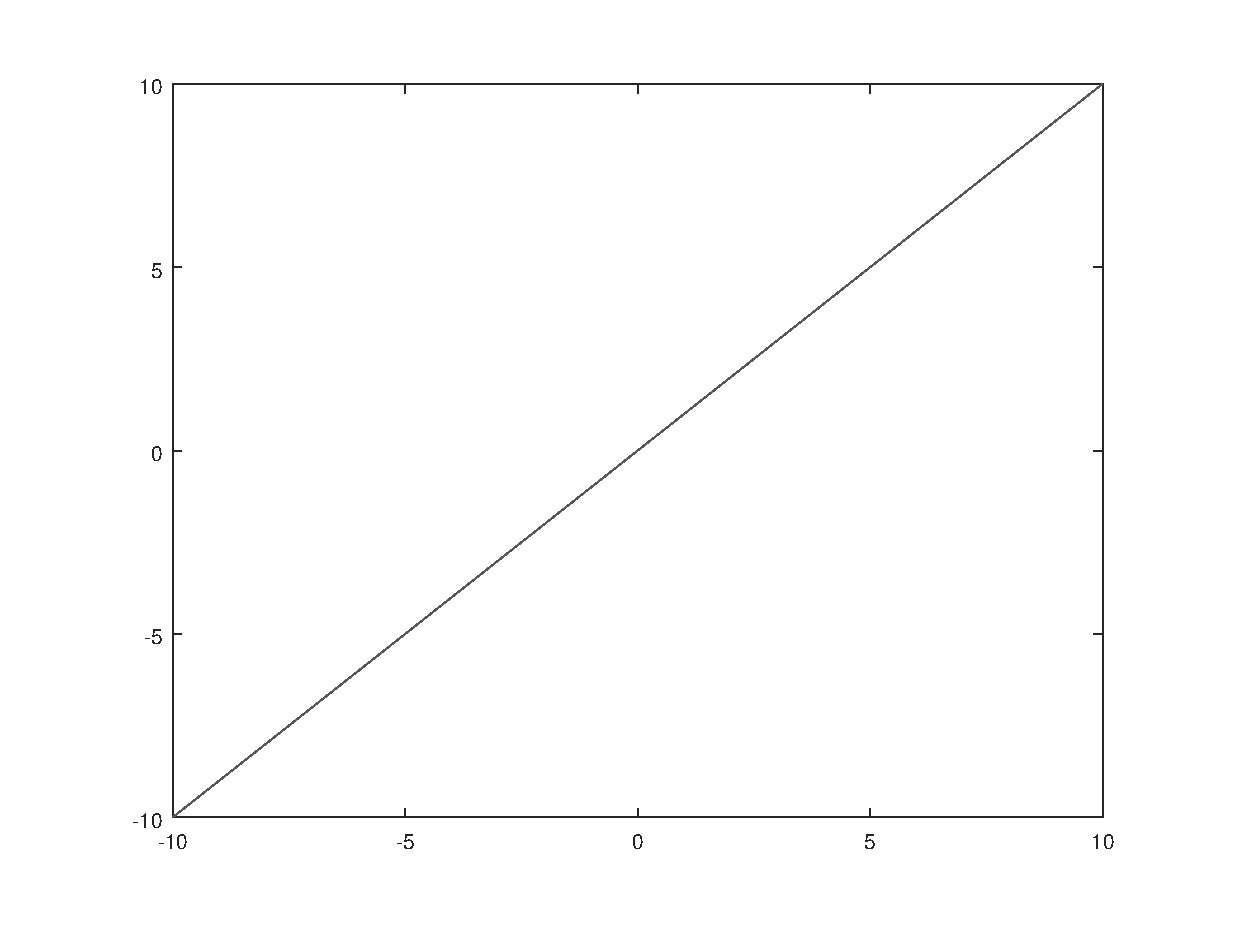
\includegraphics[width=0.9\linewidth]{img/grafica_recta.eps}
		\caption{Una recta.}
		\label{fig:sub_grafica_2}
	\end{subfigure}
	~ % No remover porque ocasionaría un salto de línea
	\begin{subfigure}[ht!]{.32\linewidth}
		\centering
		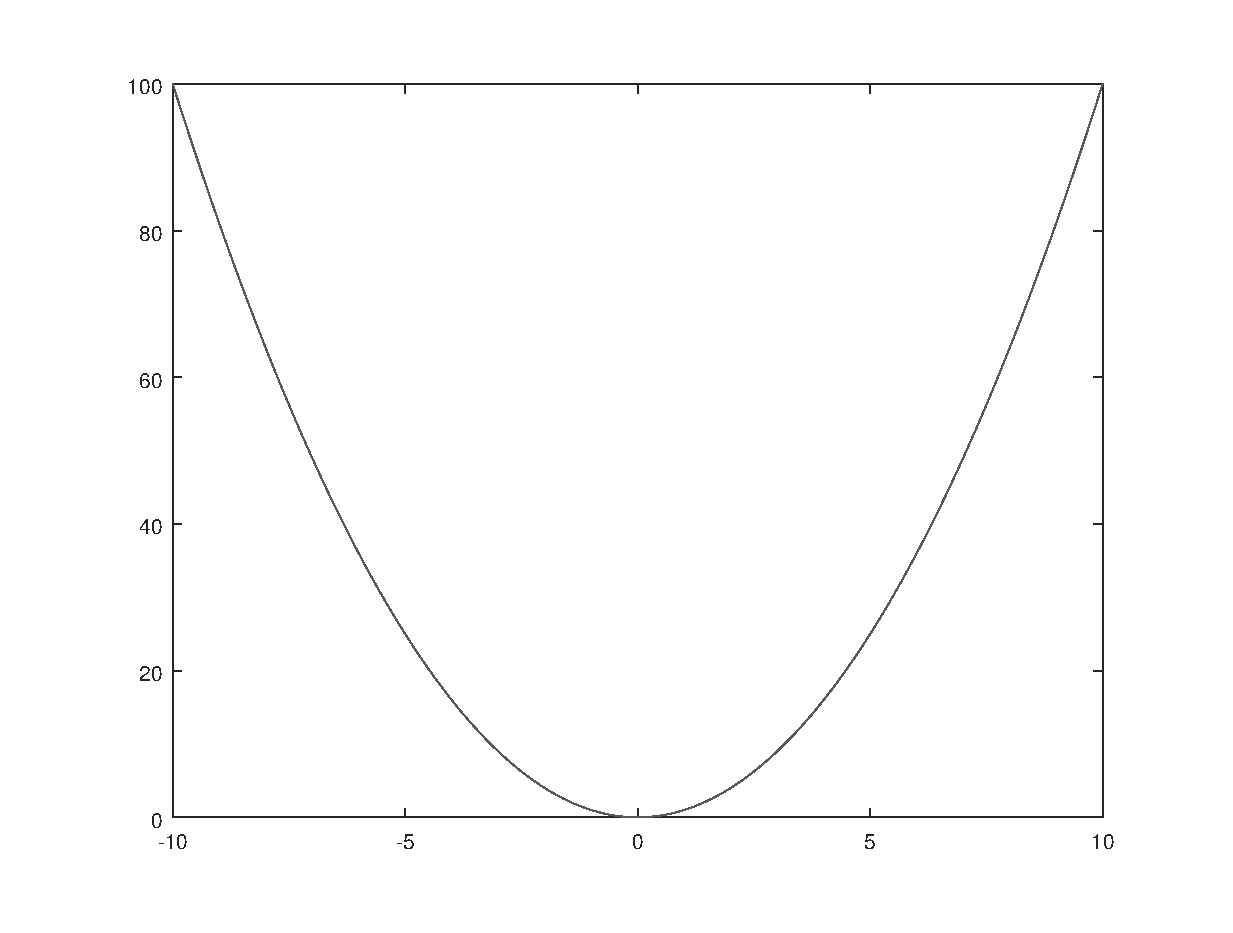
\includegraphics[width=0.9\linewidth]{img/grafica_parabola.eps}
		\caption{Una parábola.}
		\label{fig:sub_grafica_3}
	\end{subfigure}
	\caption{Tres gráficas de Octave.}
	\label{fig:tres_subfiguras}
\end{figure}

El código de la figura \ref{fig:tres_subfiguras} se muestra en el listado \ref{lst:tres_subfiguras}, donde podemos apreciar que el ancho de cada subfigura es del 32\% del ancho de línea (líneas 2, 9, y 16). Si incremento el tamaño al 33\%, las tres imágenes no caben en la misma línea.

Lo sé, lo sé, dos subfiguras al 50\% sí caben, pero tres al 33\% no... podemos discutir todo el día al respecto, o buscar la explicación pero, al final del día, lo más rápido es disminuir un poquito los porcentajes para que todo se vea bonito (de nuevo, uno no pelea con los flotantes, solo se adapta).

\begin{lstlisting}[style=latex,numbers=left,label=lst:tres_subfiguras,caption={Código para tres subfiguras.},
linebackgroundcolor={%
	\ifnum \value{lstnumber} =  2 \color{codigo_linea_resaltada}
	\else \ifnum \value{lstnumber} =  9 \color{codigo_linea_resaltada}
	\else \ifnum \value{lstnumber} = 16 \color{codigo_linea_resaltada}
	\else \color{codigo_fondo}
	\fi\fi\fi % Tantos \fi como líneas subrayadas.
}]
\begin{figure}[ht!]
	\begin{subfigure}[ht!]{.32\linewidth}
		\centering
		\includegraphics[width=0.9\linewidth]{img/grafica_seno.eps}
		\caption{Función seno.}
		\label{fig:sub_grafica_1}
	\end{subfigure}
	~ % No remover porque ocasionaría un salto de línea
	\begin{subfigure}[ht!]{.32\linewidth}
		\centering
		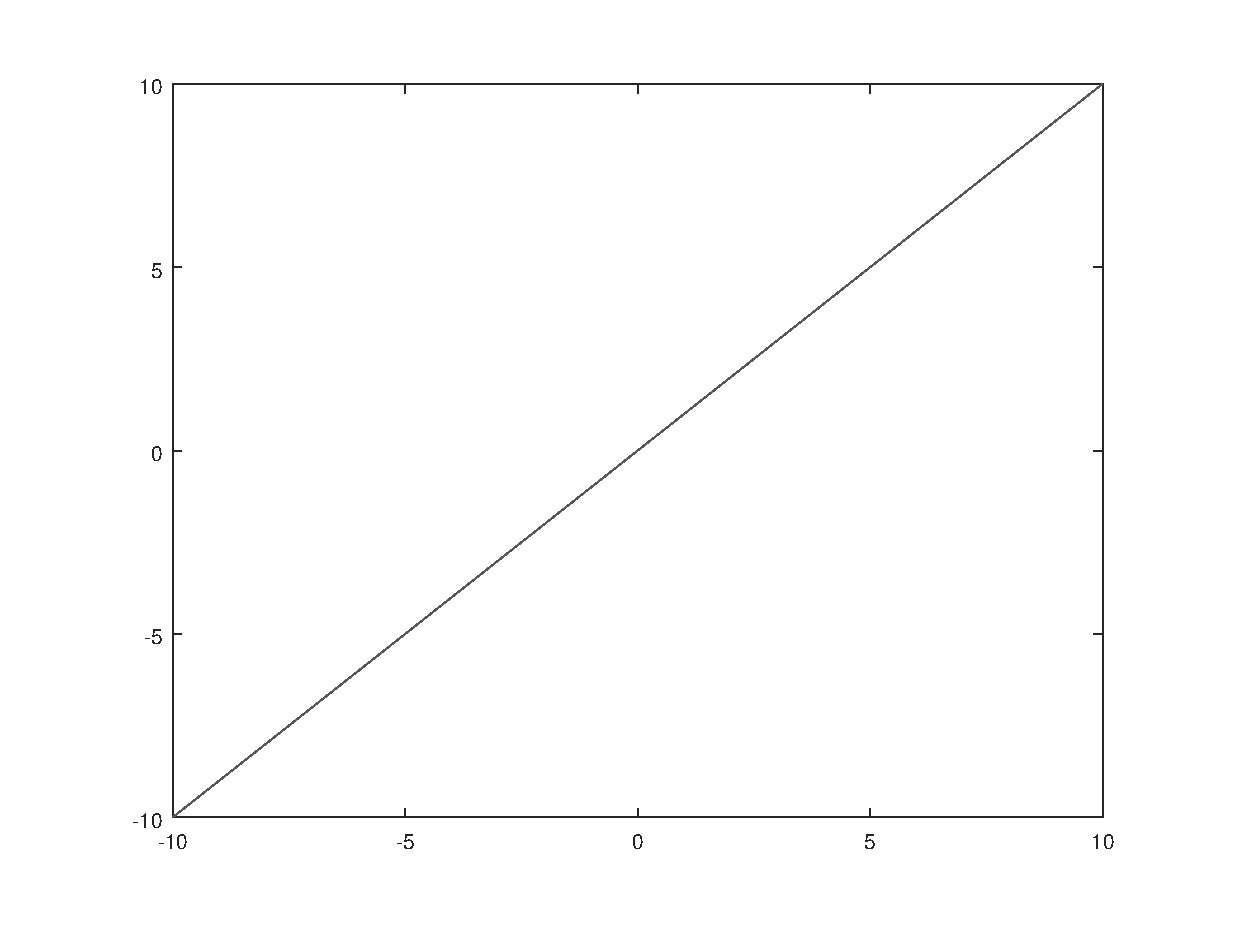
\includegraphics[width=0.9\linewidth]{img/grafica_recta.eps}
		\caption{Una recta.}
		\label{fig:sub_grafica_2}
	\end{subfigure}
	~ % No remover porque ocasionaría un salto de línea
	\begin{subfigure}[ht!]{.32\linewidth}
		\centering
		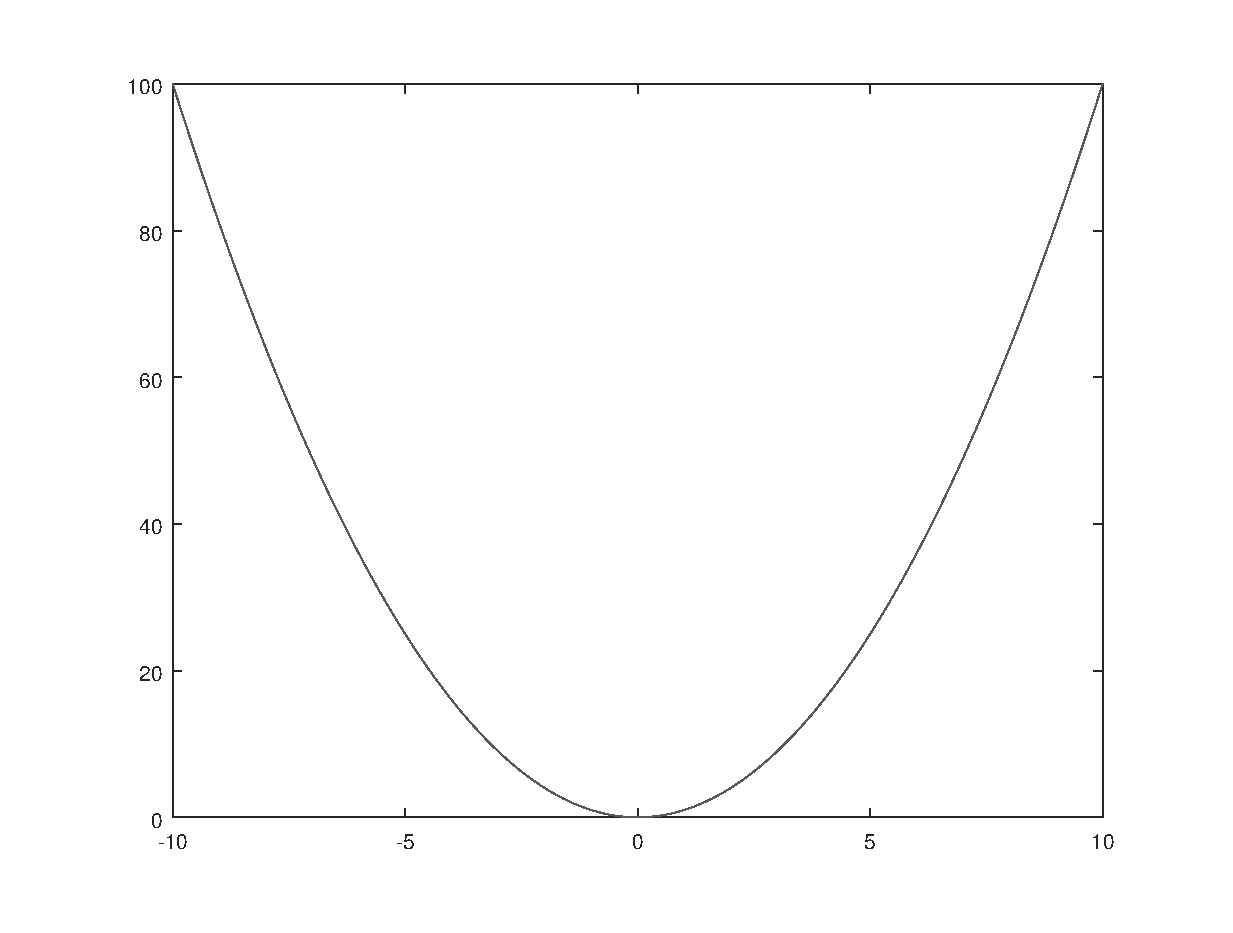
\includegraphics[width=0.9\linewidth]{img/grafica_parabola.eps}
		\caption{Una parábola.}
		\label{fig:sub_grafica_3}
	\end{subfigure}
	\caption{Tres gráficas de Octave.}
	\label{fig:figure_subfigure}
\end{figure}
\end{lstlisting}

Espero que con este ejemplo de subfiguras también te quede claro por qué \LaTeX{} no marca error al incluir varias |\caption| en un mismo entorno |figure|: hay usos legítimos que permiten este comportamiento.

Lo que el paquete |subfigure| hace es darnos una forma más fácil de trabajar con este comportamiento donde más de una etiqueta será necesaria dentro de un mismo entorno |figure|.

Y, en general, eso es lo que la mayoría de los paquetes hacen: encapsular la complejidad de \LaTeX{} con más entornos e instrucciones, para facilitarnos la vida a aquellos que no somos expertos en el tema pero deseamos hacer lo mismo.



\section*{Resumen}



En este capítulo aprendimos a ver las figuras en \LaTeX{} con nuevos ojos. Primero, aprendimos que la forma de referenciarlas el 99.9\% de las veces es a través de etiquetas y referencias.

Después, que las imágenes se incluyen gracias al paquete \texttt{graphicx}, y que se incluyen por referencia al nombre de archivo, generando peso en el documento de tesis hasta que se genera el PDF.

Investigamos varias opciones para lidiar con el tamaño de imagen, entre los que están \texttt{scale}, \texttt{width}, \texttt{height}, y \texttt{keepaspectratio}.

Finalmente, aprendimos a incluir subfiguras, que es lo mismo que decir que es una figura con varias figuritas bebé.

Pero aún queda otra especie de flotantes primitivos sin investigar: las tablas.